\documentclass[a4paper,11pt]{article}
\input{/home/tof/Documents/Cozy/latex-include/preambule_doc.tex}
\input{/home/tof/Documents/Cozy/latex-include/preambule_commun.tex}
\newcommand{\showprof}{show them}  % comment this line if you don't want to see todo environment
\setlength{\fboxrule}{0.8pt}
\fancyhead[L]{\fbox{\Large{\textbf{Algo 20}}}}
\fancyhead[C]{\textbf{Exercices parcours graphe}}
\newdate{madate}{10}{09}{2020}
%\fancyhead[R]{\displaydate{madate}} %\today
\fancyhead[R]{Terminale - NSI}
\fancyfoot[L]{\vspace{1mm}Christophe Viroulaud}
\AtEndDocument{\label{lastpage}}
\fancyfoot[C]{\textbf{Page \thepage/\pageref{lastpage}}}
\fancyfoot[R]{\includegraphics[width=2cm,align=t]{/home/tof/Documents/Cozy/latex-include/cc.png}}

\begin{document}
\begin{exo}
    La ville de Königsberg (aujourd'hui Kaliningrad) est construite autour de deux îles situées sur le Pregel et reliées entre elles par un pont.
    \begin{figure}[!h]
    \centering
    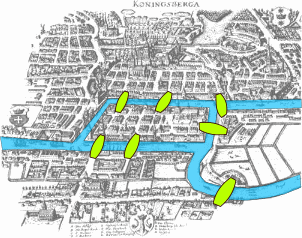
\includegraphics[width=5cm]{ressources/pont-konisberg.png}
    \captionof{figure}{Les sept ponts de Königsberg}
    \label{pont}
    \end{figure}
    
    Le problème, énoncé et résolu par Euler au XVIII° siècle, consiste à déterminer s'il existe une promenade permettant en partant d'un point, de revenir à ce même point en ayant traversé une et une seule fois chaque pont.
    \begin{enumerate}
    \item Modéliser la situation par un graphe.
    \item Tenter de réaliser la promenade \guill{à la main}.
    \end{enumerate}
    Ce problème est à l'origine de \emph{la théorie des graphes}. C'est donc Euler qui commença à théoriser des problèmes mathématiques par cette méthode. Un vocabulaire spécifique a été crée en hommage.
        \begin{aretenir}[Rappel]
            \begin{itemize}
                \item une chaîne eulérienne est une chaîne passant une et une seule fois par toutes les arêtes du graphe.
                \item un cycle eulérien est une chaîne eulérienne dont le sommet de départ et le sommet d'arrivée sont identiques. 
                \end{itemize} 
        \end{aretenir}
        \begin{aretenir}[Théorème]
            \begin{itemize}
                \item Un graphe connexe possède \textbf{une chaîne eulérienne} si et seulement si ses sommets sont tous de degré pair sauf au plus deux.
                \item Un graphe connexe possède \textbf{un cycle eulérien} si et seulement si tous ses sommets sont de degré pair. 
                \end{itemize}
        \end{aretenir}
    \begin{enumerate}[resume]
    \item Vérifier si le théorème est vrai dans le cas des ponts de Königsberg.
    \end{enumerate}
    \end{exo}
\begin{exo}
    \begin{center}
        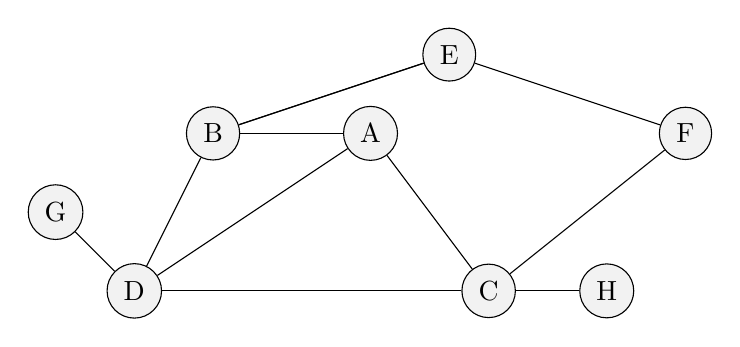
\begin{tikzpicture}
            \node[draw,circle,fill=gray!10] (A)at(0,2) {A};
            \node[draw,circle,fill=gray!10] (B)at(-2,2) {B};
            \node[draw,circle,fill=gray!10] (C)at(1.5,0) {C};
            \node[draw,circle,fill=gray!10] (D)at(-3,0) {D};
            \node[draw,circle,fill=gray!10] (E)at(1,3) {E};
            \node[draw,circle,fill=gray!10] (F)at(4,2) {F};
            \node[draw,circle,fill=gray!10] (G)at(-4,1) {G};
            \node[draw,circle,fill=gray!10] (H)at(3,0) {H};
            \draw[-,>=latex] (A) -- (B);
            \draw[-,>=latex] (A) -- (C);
            \draw[-,>=latex] (A) -- (D);
            \draw[-,>=latex] (D) -- (B);
            \draw[-,>=latex] (B) -- (E);
            \draw[-,>=latex] (B) -- (E);
            \draw[-,>=latex] (D) -- (G);
            \draw[-,>=latex] (C) -- (F);
            \draw[-,>=latex] (C) -- (H);
            \draw[-,>=latex] (C) -- (D);
            \draw[-,>=latex] (E) -- (F);
        \end{tikzpicture}
    \end{center}
    \begin{enumerate}
        \item Donner l'ordre du graphe.
        \item Donner le degré du sommet D.
        \item Construire le dictionnaire d'adjacence du graphe.
        \item Reprendre l'implémentation du parcours en profondeur vu en classe (code \ref{cours}) et remplacer le tableau \textbf{\texttt{visites}} par un dictionnaire associant chaque sommet à un booléen.
    \begin{center}
        \begin{lstlisting}[language=Python  , xleftmargin=2em, xrightmargin=2em]
def profondeur(graphe: dict, noeud: str, visites: list) -> None:
    if noeud not in visites:
        print(noeud, end=" ")
        visites.append(noeud)
        for voisin in graphe[noeud]:
            profondeur(graphe, voisin, visites)
\end{lstlisting}
                  \captionof{code}{Parcours en profondeur vu en cours}
                  \label{cours}
    \end{center}
    \item Écrire la fonction \textbf{\texttt{get\_indice(sommet: str) $\rightarrow$ int}} qui renvoie l'indice associé à chaque sommet. Par exemple, la fonction renverra \textbf{\texttt{0}} pour le sommet \textbf{\texttt{A}}.
    \item Reprendre alors l'implémentation (code \ref{cours}) en remplaçant \textbf{\texttt{visites}} par un tableau de booléens.
    \end{enumerate}

\end{exo}
\begin{exo}
    \begin{center}
        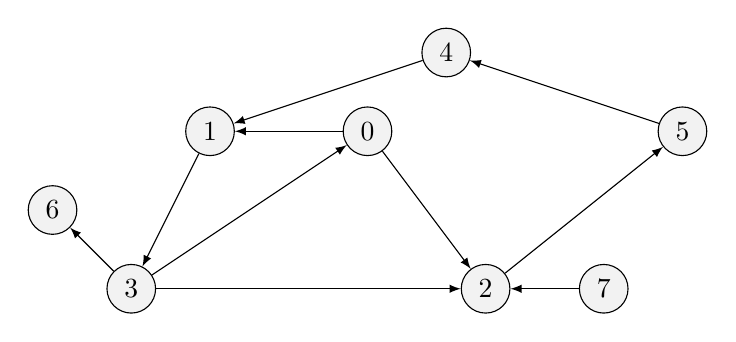
\begin{tikzpicture}
            \node[draw,circle,fill=gray!10] (A)at(0,2) {0};
            \node[draw,circle,fill=gray!10] (B)at(-2,2) {1};
            \node[draw,circle,fill=gray!10] (C)at(1.5,0) {2};
            \node[draw,circle,fill=gray!10] (D)at(-3,0) {3};
            \node[draw,circle,fill=gray!10] (E)at(1,3) {4};
            \node[draw,circle,fill=gray!10] (F)at(4,2) {5};
            \node[draw,circle,fill=gray!10] (G)at(-4,1) {6};
            \node[draw,circle,fill=gray!10] (H)at(3,0) {7};
            \draw[->,>=latex] (A) -- (B);
            \draw[->,>=latex] (A) -- (C);
            \draw[<-,>=latex] (A) -- (D);
            \draw[<-,>=latex] (D) -- (B);
            \draw[<-,>=latex] (B) -- (E);
            \draw[->,>=latex] (D) -- (G);
            \draw[->,>=latex] (C) -- (F);
            \draw[<-,>=latex] (C) -- (H);
            \draw[<-,>=latex] (C) -- (D);
            \draw[<-,>=latex] (E) -- (F);
        \end{tikzpicture}
    \end{center}
    \begin{enumerate}
        \item Construire la liste d'adjacence des successeurs du graphe.
        \item On dispose de la fonction \textbf{\texttt{parcours}}. Un sommet:
        \begin{itemize}
            \item \textbf{\texttt{BLANC:}} n'a pas encore été atteint,
            \item \textbf{\texttt{GRIS:}} est en cours de visite,
            \item \textbf{\texttt{NOIR:}} a terminé son parcours.
        \end{itemize}
        Le tableau \textbf{\texttt{visites}} associe à chaque sommet, son état \textbf{\texttt{coul}} et son prédécesseur \textbf{\texttt{pred}}.
        \begin{lstlisting}[language=Python  , xleftmargin=1em, xrightmargin=1em]
BLANC, GRIS, NOIR = 0, 1, 2

def parcours(graphe: list) -> list:
    visites = [{"coul": BLANC, "pred": None} for i in range(len(graphe))]
    for i in range(len(graphe)):
        if visites[i]["coul"] == BLANC:
            dfs(graphe, i, visites)
    return visites
\end{lstlisting}
Écrire la fonction \textbf{\texttt{dfs(graphe: list, sommet: int, visites: list) $\rightarrow$ None}} qui effectue récursivement le parcours en profondeur du \textbf{\texttt{sommet}}. La fonction utilisera le principe des trois couleurs et associera le prédécesseur de chaque voisin.
    \end{enumerate}
\end{exo}
\end{document}